\section{Modelos de Comprensión de Programas}

Generalmente se establece que la \textit{comprensión}, dentro de este ámbito de estudio, es un
proceso en el que el individuo construye su propia representación mental de un programa.
Los modelos de comprensión de programas son teorías sobre el proceso cognitivo que llevan
adelante los programadores para obtener esta representación mental.

Si bien existen varias escuelas de pensamiento, independientemente de las diferencias, la
mayoría de los modelos de comprensión de programas contiene un conjunto común de elementos,
tal como se puede ver en la Figura X \cite{SchulteClear10}.

\begin{figure}[H]
    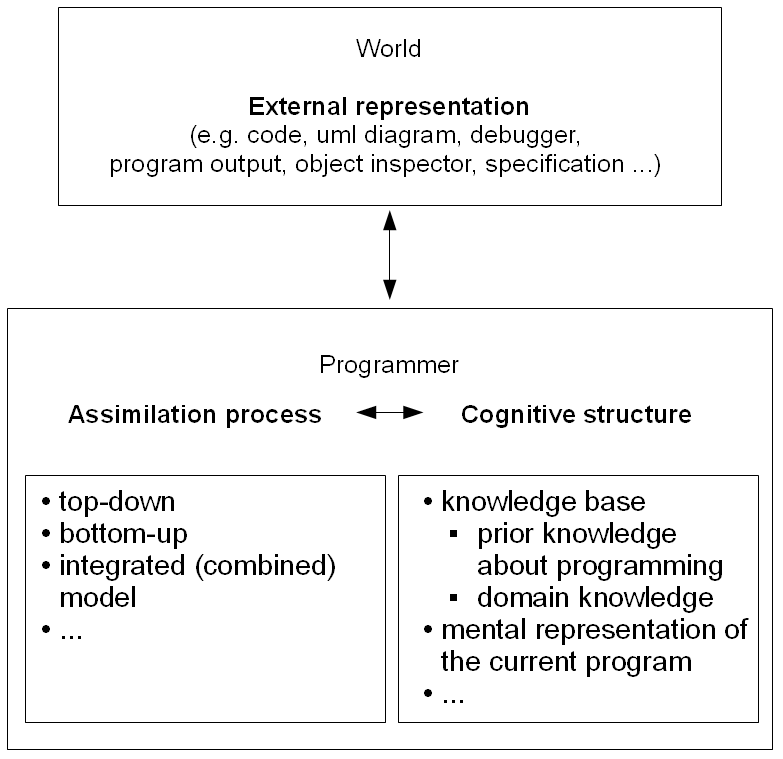
\includegraphics[width=10cm]{program_comprehension/elements.png}
    \centering
    \caption{Elementos principales de los modelos de comprensión de programas}
\end{figure}

\subsection{Representación Externa}
Se considera que la representación externa son todos aquellos materiales asociados al programa
en estudio que el programador puede utilizar para su proceso de comprensión, pero que no son 
parte del conocimiento interno del individuo.
Estos elementos pueden ser presentados de diversa forma, desde directamente el código fuente
o binarios, hasta manuales, documentación, diagramas UML, entre otros.

\subsection{Estructura Cognitiva}
El conocimiento interno de un programador, el cual puede dividirse entre \textit{base de conocimiento}
y \textit{representación mental}, es lo que se define como estructura cognitiva.

La base de conocimiento viene dada por el conocimiento general que el programador posee,
independiente de la aplicación específica que se está tratando de comprender.
Esto incluye conocimiento general de lenguajes y principios de programación, algoritmos, 
aplicaciones similares y demás.

El modelo mental es una representación interna al programador del software bajo consideración.
Determina el nivel de conocimiento del individuo sobre el sistema en cuestión, y es construido
a medida que se comprende, utilizando la base de conocimiento mencionada anteriormente.
Diferentes elementos, tanto estáticos como dinámicos, forman parte del modelo y permiten
su evolución \cite{MayrhauserVans95}.

\subsection{Proceso de Asimilación}
La estrategia implementada por los desarrolladores para extraer información de un programa, 
construir una representación mental del mismo, y así lograr su comprensión, es lo que se
conoce como proceso de asimilación.
Existen diferentes escuelas de pensamiento que han ido formulando diversos modelos, los
cuales pueden agruparse de la siguiente manera.

\begin{description}
    \item[Comprensión Top-down] Los modelos de comprensión top-down son aquellos que 
    implican la aplicación de conocimiento sobre el dominio del programa y la correlación 
    de este conocimiento con el código fuente del mismo.
    En el modelo de Brooks \cite{Brooks93}, una sucesión de hipótesis forma el proceso de asimilación.
    En el esquema de Soloway y Erlich \cite{SolowayErlich84}, los programadores utilizan planes y reglas de programación
    para descomponer objetivos y planes en otros planes de menor abstracción.
     
    \item[Comprensión Bottom-up] Caen dentro de esta clasificación aquellos modelos en
    los que su proceso de asimilación comienza con las sentencias de código fuente, y
    las mismas se van agrupando para obtener mayores niveles de abstracción.
    El proceso se repite una y otra vez, hasta lograr una representación mental completa
    del programa en cuestión.
    En el proceso de asimilación propuesto por Pennington \cite{Pennington87,Pennington87b}, 
    se presentan dos modelos diferentes.
    El modelo del programa, que se obtiene de agrupar microestructuras en macroestructuras, y
    se corresponde con una abstracción del flujo de control del programa.
    El modelo de situación, incluye el flujo de datos dentro del programa, y representa la
    función y objetivos del mismo.
    En el modelo de Shneiderman y Mayer \cite{ShneidermanMayer79}, la base de conocimiento se compone tanto de
    conocimiento sintáctico como semántico.
    A mayor experiencia del desarrollar, mayor será este último.

    \item[Estrategias Oportunistas] Algunos autores consideran que, dependiendo
    de la necesidad de comprensión para la tarea en cuestión, no existe un enfoque
    sistemático de resolución, por lo que un programador puede aprovechar tanto
    las estrategias bottom-up como top-down.
    Letovsky \cite{Letovsky87} plantea que un programador puede procesar la información 
    de forma bottom-up o top-down a medida que van apareciendo pistas que ayuden a su comprensión.
    Littman \cite{LittmanPinto87} propone que un programador toma un enfoque de acuerdo
    a la necesidad, u oportunista, en constraste con un enfoque más sistemático,
    sin el requerimiento de lograr un modelo mental completo del sistema.
    
    \item[Modelos Integrados] Los modelos integrados \cite{MayrhauserVans95} suponen 
    una combinación de los anteriores, en donde el proceso de asimilación implica ir cambiando 
    de modelos a medida que se requiera, para poder construirlos simultáneamente.
    Se plantean tres representaciones mentales: el modelo del dominio, el modelo del
    programa y el modelo de situación.
    Es muy importante la base de conocimiento del programador, ya que le va a permitir
    la construcción de las representaciones.

\end{description}
